\chapter{ESTRUCTURA DE UN COMPILADOR}
\section{COMPILADORES Y TRADUCTORES}
\section{ESTRUCTURA TÍPICA DE UN COMPILADOR}
\begin{figure}[H]
    \centering
    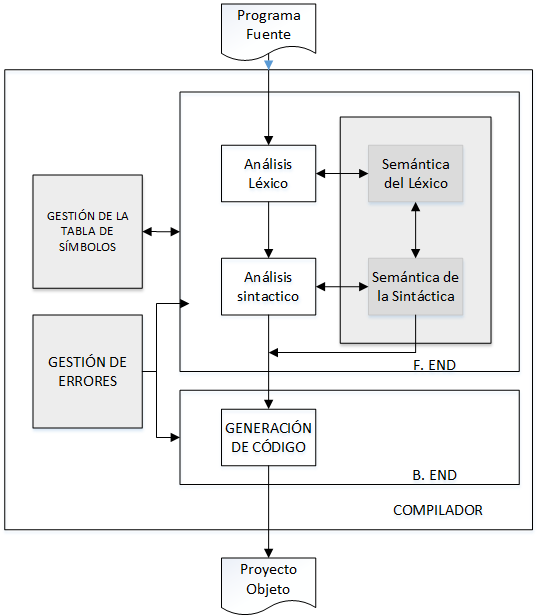
\includegraphics[width=0.8\textwidth, height=10cm,keepaspectratio]{chapters/chapter1/figures/Fig1 Estructura del compilador.png}
    \caption{Caption}
    \label{fig:my_label}
\end{figure}

\begin{figure}[H]
    \centering
    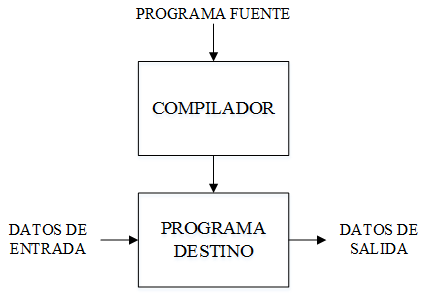
\includegraphics[width=0.8\textwidth, height=10cm,keepaspectratio]{chapters/chapter1/figures/Fig2 Flujo Programa.png}
    \caption{Caption}
    \label{fig:my_label}
\end{figure}


\subsection{ANÁLISIS LÉXICO}



\begin{figure}[H]
    \centering
    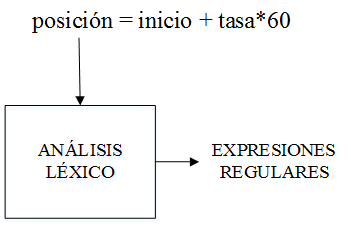
\includegraphics[width=0.8\textwidth, height=10cm,keepaspectratio]{chapters/chapter1/figures/Fig3 Analisis Lexico.png}
    \caption{Caption}
    \label{fig:my_label}
\end{figure}
\subsection{ANÁLISIS SINTÁCTICO}
\begin{figure}[H]
    \centering
    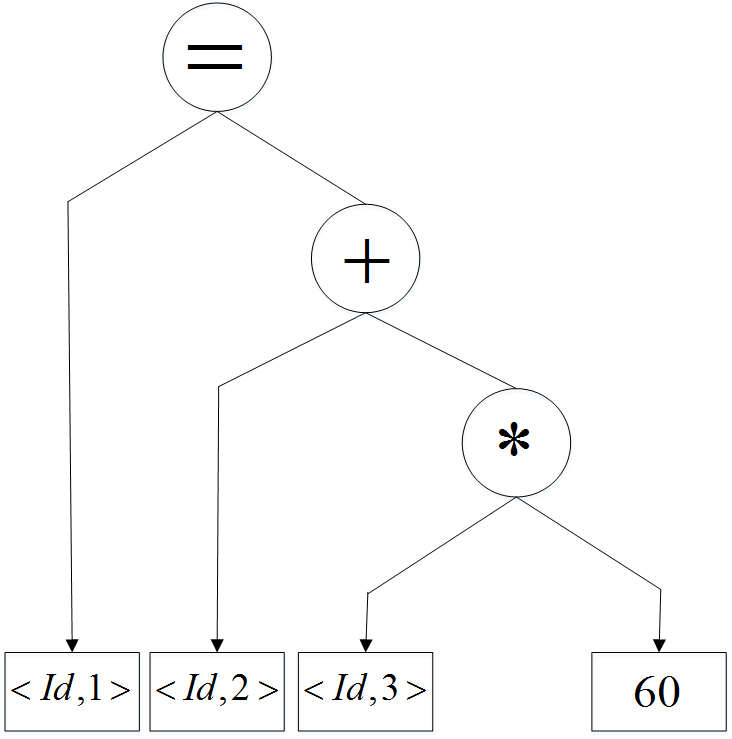
\includegraphics[width=0.8\textwidth, height=10cm,keepaspectratio]{chapters/chapter1/figures/Fig4 Analisis Sintactico.png}
    \caption{Caption}
    \label{fig:my_label}
\end{figure}

\subsection{ANÁLISIS SEMÁNTICO}
\begin{figure}[H]
    \centering
    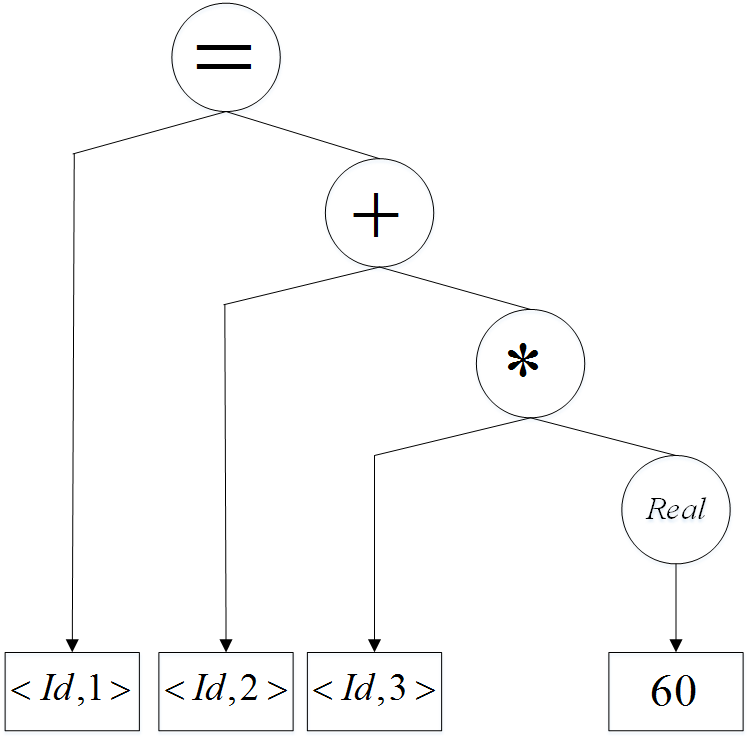
\includegraphics[width=0.8\textwidth, height=10cm,keepaspectratio]{chapters/chapter1/figures/Fig5 Analisis Semantico.png}
    \caption{Caption}
    \label{fig:my_label}
\end{figure}
\subsection{GENERACIÓN DE CÓDIGO}

\subsection{TABLA DE SÍMBOLOS Y MANEJO DE ERRORES}
\section{HERRAMIENTAS DE APOYO EN LA CONSTRUCCIÓN DE COMPILADORES} \label{sec:herraminetasConstruccionCompiladores} 
\begin{itemize}
    \item Herramientas de Software
    \item Generadores de analizadores léxicos LEX
    \item Generadores de analizadores sintácticos YACC
    \item Monitores de traducción DIRI por sintaxis YACC
    \item Generadores de generadores de código
    \item Monitores de análisis de flujo de datos
    \item Toolkits para construcción de compiladores TOOLS
\end{itemize}
\section{COMPILADORES Y COMPUTACIÓN}

\begin{enumerate}
    \item Programa fuente \\
    \begin{align*}
        posición:=inicio+velocidad * 60
    \end{align*}
    \item Resultados de análisis léxico \\
     \begin{align*}
        & \langle id_1, `posición` \rangle\\
        & \langle OperAsig, `:=` \rangle\\
        & \langle id_2, `inicio` \rangle\\
        & \langle OperAdic, `+` \rangle\\
        & \langle id_3, `velocidad` \rangle\\
        & \langle OperadorMul, `*` \rangle\\
        & \langle Const, `60` \rangle\\
    \end{align*}
    $ \boxed{id_1:=id_2+id_3\times 60} $ \\
    \item Análisis sintáctico\\
    \item Análisis semántico\\
    \item Generación de código intermedio\\
    No esta asociado a ninguna maquina especifica. En principio es equivalente a las acciones que el programador quiere realizar en el lenguaje de alto nivel.\\
    Existen estandares establecidos sobre los codigos intermedios mas usados\\
    \begin{align*}
        & temp1:=enteroreal(60) \\
        & temp2:=id3 * temp1 \\
        & temp3:=id1 + temp2 \\
        & id1:=temp3 \\
    \end{align*}
    \item Optimización de código\\
    \begin{align*}
        & temp1:=id3*60.0 \\
        & id1:=id2+temp1 \\
    \end{align*}
    \item Generación de código ensamblador \\\\
    Muy ligado al fabricante\\
    
    MOVF id3, R2 \\
    MULF #60.0, R2 \\
    MOVF id2, R1 \\
    ADDF R2, R1 \\
    MOVF R1, id1 \\



\end{enumerate}

\section{EJERCICIOS DEL CAPÍTULO}
\begin{enumerate}
    \item De la recursión:
        \begin{enumerate}
            \item Realizar los diseños necesarios para la implementación del concepto de recursión se pueda realizar en un lenguaje que no tenga esta característica
            \item Implementar el caso particular con el algoritmo de Euclides.
        \end{enumerate}
    \item Hacer la  estimación de la complejidad del algoritmo de Euclides
\end{enumerate}
\section{RESUMEN Y PANORAMA HISTÓRICO}
\subsection{RESUMEN}
\subsection{PANORAMA HISTÓRICO}
\section{REFERENCIAS BIBLIOGRÁFICAS}